
Most optimization problems are NP-complete, and therefore cannot be solved directly
at low cost. As a solution, we can use a simplified version of the problem which
would be easier to solve (by, for instance, releasing constraints). But when
translating the optimum of the simplified problem back to the original setting, we
have no guarantee that the optimality is preserved. We can therefore wonder how far
this rounded optimum is from the actual optimum. Bounding this distance will enable
us to link the obtained optimum to the one of the first problem. We will focus in
this chapter on the Max-SAT problem.\\

\begin{center}
 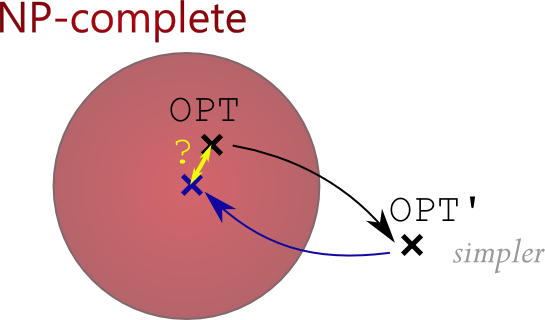
\includegraphics[width=0.6\textwidth]{Figures/img1}
\end{center}



%\subsection{Derandomizing MAX-SAT using Conditional Expectation}
\subsection{Approximation algorithms for Max-SAT}
Max-SAT is the typical problem in order to study results about approximations.\\

\textbf{Max-SAT}\\
Given a boolean formula $\phi$ on $x_1, \dots, x_n$ written in Conjunctive Normal
Form, $\displaystyle \phi = \bigwedge_{j=1}^m{C_j}$ where clauses $\displaystyle
C_j=\bigvee_{k=1}^{l_j}{L_k}$,
$L_k\in \{x_i, \neg x_i\}$, the problem is to compute the maximum number of clauses
an assignment on the $x_i$ can satisfy.\\

The SAT problem, which is NP-complete, is clearly a particular case where all the
clauses are satisfied: unless P=NP, there is no algorithm that can decide in polynomial time
whether Max-SAT = $m$ or not. The fact to distinguish between $(m-1)$ and $m$
satisfied clauses is therefore NP-complete. The PCP theorem enables to widen this
result: being able to distinguish between $(\frac{7}{8}+\epsilon)m$ and $m$
satisfied clauses would mean being able to solve any NP problem. That is why, $\forall\epsilon>0$, there
is no  $(\frac{7}{8}+\epsilon)$-approximation for this problem. Note
that the result also stands when all the clauses have length 2, but the constant
$\frac{7}{8}$ is specific to clauses of length 3.

\begin{center}
 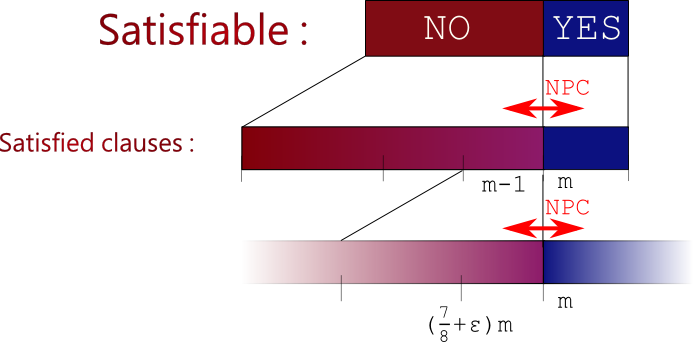
\includegraphics[width=0.6\textwidth]{Figures/img2}\\
\end{center}

Randomization does not seem to have a huge impact on such problems: the speedup is
limited, because most randomized algorithm have inspired deterministic equivalent
solutions. As a general rule, if there exists a very hard problem, we can use it to
generate pseudorandom strings, which we can then use to derandomize any randomized
algorithm, limiting the impact of randomization. In the other case, we can show that
the permanent is hard to compute. \\




%\subsubsection{Randomized algorithm}

Let us consider MAX-SAT has $m$ clauses with each clause $C_j$ having $l_j$ literals in it. Let the MAX-SAT
function be denoted by $\phi$. Let us assume the literal $x_i$ is $true$ in the original MAX-SAT $\phi$ gets transformed to  $\phi_i^0$ 
and similarly $\phi_i^1$ when we assume $x_i$ is false.

Let us consider an assignment on the $x_i$, and let $y_1, \dots, y_n$ and $Z_1, \dots,
Z_m$ be variables in $\{0,1\}$ such that:
\begin{align*} 
y_i &= \left\{ \begin{array}{l l}
    1 & \quad \text{if $x_i$ is true}\\
    0 & \quad \text{if $x_i$ is false}\\
\end{array} \right. \\   
Z_j &= \left\{ \begin{array}{l l}
    1 & \quad \text{if the clause $C_j$ is satisfied}\\
    0 & \quad \text{otherwise}\\
\end{array} \right.
\end{align*} 

We use the notation $L_j^+ = \{ i : x_i \in C_j \}$ and $L_j^- = \{ i | \bar{x_i} \in C_j \}$ where $C_j$ is a clause and $x_i$ is a literal.

\subsubsection{Algorithm 1 - Random Assignment + Derandomization}
%Random assignment should be the lower bound for the performance of any algorithm proposed because 
%it is the simplest possible way of solving a problem. 
%\begin{eqnarray}
%E(\mbox{cost(Algorithm 1)}) =  \sum_{j=1}^m E(z_j) = \sum_{j=1}^m Pr(z_j = 1) = \sum_{j=1}^m 1 - \frac{1}{2^{l_j}} \geq (1 - \frac{1}{2^{l_{min}}}).m \nonumber
%\end{eqnarray}
%where $l_{min} =$ size of the smallest clause in the MAX-SAT.

The easiest solution to this problem is to try random assignments.\\
Since a clause is satisfied if at least one of its $l$ literals is true, the
probability for a single clause to be satisfied by a random assignment (none of the
literals are true) is: 
\[\mathbb{P}=1-\left( \frac{1}{2} \right)^l\]
%For each such clause, we will introduce a random variable $Z_j$ which will be worth
%1 if the random assignment satisfies the clause $C_j$, or 0 otherwise.\\
Hence, the expected result of such a random algorithm, that is to say the expected
number $\mathbb{E}$ of satisfied clauses, is:
\[\mathbb{E} = \sum_{j=1}^{m}{\mathbb{E}[Z_j]} = \sum_{j=1}^{m}{1 \times \left(
1-\left( \frac{1}{2} \right)^l \right)} 
\geq m \times \left( 1-\left( \frac{1}{2} \right)^{l_{min}} \right)\]
By linearity of expectation and with $l_{min} = \min (l_j)$\\
If all the clauses have at least 3 literals, this last term is worth $\frac{7}{8}$:
$\mathbb{E} \geq \frac{7}{8} m$: it is therefore optimal. But this algorithm is very
bad if there exist a clause with a few number of literals (if there is a clause with
1 literal, we can only guarantee that half the clauses will be satisfied). This is
the case that needs improving.

	\paragraph{Derandomization}
Using cost of expectation of the algorithm in equation-\label{algo-1} we can derandomize this algorithm in the following way. Let us consider a literal $x_i$. 
\begin{eqnarray}
E(\mbox{cost(Algorithm1)}) & = & E(\mbox{cost(Algorithm1)} | y_i = 0) Pr(y_i = 0) \nonumber \\
                            & + &E(\mbox{cost(Algorithm1)} | y_i = 1) Pr(y_i = 1) \nonumber
\end{eqnarray}
which is using the average of the Expectation of the algorithm conditioned on literal $y_i$. Instead if we consider to assign a
value to $y_i$ a value which maximizes using the conditional expectation i.e. $\max_a E(\mbox{cost(Algorithm1)} | y_i = a)$
where $ a \in \{0,1\}$.

The expectations conditioned on variable $y_i$ can be calculated as  
\begin{eqnarray}
E(\mbox{cost(Algorithm1)} | y_i = 0) & = &\sum_{C_j \in \phi_i^0} ( 1 - \frac{1}{2^l_j}) \nonumber \\
E(\mbox{cost(Algorithm1)} | y_i = 1) & = &\sum_{C_j \in \phi_i^1} ( 1 - \frac{1}{2^l_j}) \nonumber
\end{eqnarray}
The above costs can be calculated deterministically in polynomial time. Hence we greedily assign $y_i$ the value that increases the expected cost of
the algorithm.


\subsubsection{Algorithm 2 - Linear Programming + Derandomization}

Max-SAT is equivalent to the following linear problem (with the previous definitions):

\begin{eqnarray}
MAXSAT(\phi) & = &\max \sum_{j=0}^m z_j \nonumber \\
&\forall Z_j,~Z_j \leq &\sum_{i \in L_j^+} y_i + \sum_{i \in L_j^-} (1 - y_i) \nonumber \\
&\forall j,~ z_j \in \{0, 1\} \nonumber \\
&\forall i,~  y_i \in \{0, 1\} \nonumber 
\end{eqnarray}

Unfortunately, we do not know any polynomial algorithm able to solve such a linear
problem. But, if we replace the conditions $y_i \in \{0,1\}$ and $z_j \in \{0,1\}$
by the conditions $y_i, z_j \in \mathbb{R}$ and $0 \le y_i, z_j \le 1$, this problem
can be solved in polynomial time (for example using the ellipsoid algorithm of
Khachiyan). Let $OPT$ be the maximum value for the original problem and $OPT_f$ be
the one for the problem with real variables (clearly $OPT_f \ge OPT$). Using this
technique, we can propose the following algorithm:


\begin{theorem}[{\bf An algorithm based on linear programming}]
~
\begin{enumerate}
\item Compute an optimal solution for the above problem with variables in $[0,1]$.
Let $y^*_1, \dots, y^*_n$, $z^*_1, \dots, z^*_m$ this solution.
\item Set $x_i = 1$ with probability $y^*_i$ (independently).\\
\end{enumerate}
The proposed algorithm is so a $(1 - \frac{1}{e})$-randomized approximation for
Max-SAT.
\end{theorem}

The expected number $\mathbb{E}$ of satisfied clauses, is:
\[ \mathbb{E} = \sum_{j=1}^{m}{\mathbb{E}[Z_j]} \]
(as in the previous subsection, we define $Z_j = 1$ if and only if the clause $C_j$ is
satisfied)

Without loss of generality, we can renumber the variables and replace $x_i$ by $\neg
x_i$ such that:
\[ C_1 = x_1 \vee \dots \vee x_l \]
where $l = l_1$.

Then:
\begin{align*}
\mathbb{P} (Z_1 = 1) &= 1 - \mathbb{P} \left( \bigcap_{i=1}^l \{ x_i = 0 \} \right) \\
&= 1- \prod_{i=1}^l \mathbb{P}(x_i = 0) \quad \text{by independence of the $x_i$} \\
&= 1 - \prod_{i=1}^l (1 - y^*_i)
\end{align*}

Since the logarithm function is concave: for all $a_1, \dots, a_l \in \mathbb{R^*_+}$:
\begin{align*}
\frac{1}{l} \sum_{i=1}^l \log a_i \; &\le \; \log \left( \sum_{i=1}^{l}
\frac{a_i}{l} \right) \\
\prod_{i=1}^l a_i \; &\le \; \left( \sum_{i=1}^{l} \frac{a_i}{l} \right) ^ l
\end{align*}

And so:
\[
\mathbb{P} (Z_1 = 1) \ge 1 - \left( \sum_{i=1}^{l} \frac{1 - y^*_i}{l} \right) ^
l = 1 - \left(1 - \sum_{i=1}^{l} \frac{y^*_i}{l} \right) ^ l 
\]

But we also have: $z^*_1 \le \sum_{i=1}^{l} y^*_i$ since the $y^*_i$ and the $z^*_j$
verify the constraint of the previous linear problem. Hence:
\begin{equation} \label{eq:probaZ1}
 \mathbb{P} (Z_1 = 1) \ge 1 - \left( 1 - \frac{z_1}{l} \right)^l
\end{equation}

Let $g : \left( \begin{array}{l c l}
    [0,1] & \rightarrow & \mathbb{R}\\
    x & \mapsto & 1- (1-\frac{z}{l})^l - (1-\frac{1}{e}) z
    \end{array} \right)$
    
If $l=1$, $g(z) = 1 \ge 0$. Otherwise $l \ge 2$ and:
\begin{align*}
g'(z) &= \left( 1 - \frac{z}{l} \right)^{l-1} - \left(1 - \frac{1}{e} \right) \\
g''(z) &= \frac{l-1}{l} \left( 1 - \frac{z}{l} \right)^{l-2} \ge 0
\end{align*}
$g$ is then concave and so its minimum is either $g(0) = 1$ or $g(1)$. And, since
the logarithm function is concave:
\begin{equation} \label{eq:classicIneq}
 \left(1 - \frac{1}{l}\right)^l = e^{l \log(1-\frac{1}{l})} \le e^{-\frac{l}{l}} =
\frac{1}{e} 
\end{equation}

This means $g(1) = 1- (1-\frac{1}{l})^l - (1-\frac{1}{e}) \ge 0$ and so $g(z) \ge 0$
for all $z \in [0,1]$.

Hence, according to equation~\eqref{eq:probaZ1}:
\[ \mathbb{P} (Z_1 = 1) \ge g(z^*_1) + \left( 1 + \frac{1}{e} \right) z^*_1 \ge
\left( 1 - \frac{1}{e} \right) z^*_1 \]

and:
\[ \mathbb{E} \ge \sum_{j=1}^m \left( 1 - \frac{1}{e} \right) z^*_j = \left( 1 -
\frac{1}{e} \right) OPT_f \ge \left( 1 - \frac{1}{e} \right) OPT \]

The proposed algorithm is so a $(1 - \frac{1}{e})$-randomized approximation for
Max-SAT. This is better than the first algorithm only for small clauses (when
$l_{min} = 1$, $1 - \frac{1}{e} \ge 1 - \frac{1}{2^{l_{min}}}$).

\paragraph{Derandomization}
We can derandomize this algorithm also similar to the derandomizing the above Algorithm-1 by calculating the conditional expectations and assigning the 
value which fetches maximum expected cost.
\begin{eqnarray}
E(\mbox{cost(Algorithm2)} | y_i = 0) & = &\sum_{C_j \in \phi_i^0} ( 1 - \prod_{i\in L_j^+}(1 - y_i^*) \prod_{i \in L_j^-} y_i^*) \nonumber \\
E(\mbox{cost(Algorithm2)} | y_i = 1) & = &\sum_{C_j \in \phi_i^1} ( 1 - \prod_{i\in L_j^+}(1 - y_i^*) \prod_{i \in L_j^-} y_i^*) \nonumber
\end{eqnarray}


\subsubsection{Combining both}

The first algorithm behaves better with clauses with a lot of literals whereas the
second one behaves better with clauses with few literals. Therefore it would be good
to combine this two algorithms.

An idea is to choose randomly the algorithm to run: run
the first one with probability $p$ and the second one with probability $1-p$ ($p$
will be fixed later).

In this case we have:
\[
\mathbb{E} = \sum_{j=1}^{m}{\mathbb{P}(Z_j = 1)}
\]
and:
\begin{align*}
\mathbb{P}(Z_j = 1) &\ge p \left( 1 - \frac{1}{2^{l_j}} \right) + (1-p) \left( 1 -
\left(1-\frac{1}{l_j}\right)^{l_j} \right) \\
&\ge 1 - p \frac{1}{2^{l_j+1}} - (1-p) \left(1-\frac{1}{l_j}\right)^{l_j} = p_j
\end{align*}

\begin{itemize}
\item if $l_j = 1$, $p_j = 1 - \frac{p}{2}$ and $p_j \ge \frac{3}{4}$ if $p \le
\frac{1}{2}$.
\item if $l_j = 2$, $p_j = 1 - \frac{p}{4} - \frac{1-p}{4} = \frac{3}{4}$.
\item if $l_j \ge 3$ and $p= \frac{1}{2}$:
\[ p_j = 1 - \frac{1}{2^{l+1}} - \frac{1}{2} \left( 1 - \frac{1}{l} \right)^l \ge 1
- \frac{1}{2^4} - \frac{1}{2}\frac{1}{e}  \approx 0.753 \ge \frac{3}{4}\]
(the first inequality comes from the equation~\eqref{eq:classicIneq}
page~\pageref{eq:classicIneq})
\end{itemize}

The goal is to maximize over $p$ the minimum over $l_j$ of $p_j$. Since if $l_j =
2$, $p_j = \frac{3}{4}$, necessarily this minimum over $l_j$ is greater or equal
than $\frac{3}{4}$. Furthermore with $p=\frac{1}{2}$, the result minimum is
$\frac{3}{4}$. So set $p=\frac{1}{2}$.

Therefore, this final algorithm is a $\frac{3}{4}$-random approximation of the Max-SAT
problem (which is better than the two other algorithms when $l_{min} = 1$).

But this could still be improved by running the two first algorithms and taking the
best result. The resulting algorithm will be at least a $\frac{3}{4}$-random
approximation of the Max-SAT problem for $l_{min} = 1$ and a $(1 -
\frac{1}{2^{l_{min}}})$-random approximation otherwise.
